%%%%%%%%%%%%%%%%%%%%%%%%%%%%%%%%%%%%%%%%%%%%%%%%%%%%%
%                                                   %
%     Penn State Colloquium Poster Template         %
%                                                   %
% Uses Penn State Colloquium class, with options:   %
%                                                   %
% Orientation:                                      %
%     portrait (default), landscape                 %
%                                                   %
% Paper size:                                       %
%     a4paper (default), a0paper, a1paper, a2paper, %
%     a3paper, a5paper, a6paper                     %
%%%%%%%%%%%%%%%%%%%%%%%%%%%%%%%%%%%%%%%%%%%%%%%%%%%%%
\documentclass{../psuposter}
\renewcommand{\templateimagepath}{../} 


%%%%%%%%%%%%%%%%%%%%%%%%%%%%%%%%%%%%%%%%%%%%%%%%%%%%%
%               Package Dependencies                %
%%%%%%%%%%%%%%%%%%%%%%%%%%%%%%%%%%%%%%%%%%%%%%%%%%%%%
\usepackage{natbib}
\usepackage{lipsum}                                % Dummy text
\usepackage[figwidth = 0.98\linewidth]{todonotes}  % Dummy image (and more!)
\usepackage[absolute, overlay]{textpos}            % Figure placement
\usepackage{braket}
\setlength{\TPHorizModule}{\paperwidth}
\setlength{\TPVertModule}{\paperheight}
\setcitestyle{numbers,square}


%%%%%%%%%%%%%%%%%%%%%%%%%%%%%%%%%%%%%%%%%%%%%%%%%%%%%
%                 AUTHOR AND TITLE                  %
%%%%%%%%%%%%%%%%%%%%%%%%%%%%%%%%%%%%%%%%%%%%%%%%%%%%%
\title{Chiral Symmetry and Topological Insulators in Particle Physics}
\author{David B. Kaplan}
\institute{University of Washington}


%%%%%%%%%%%%%%%%%%%%%%%%%%%%%%%%%%%%%%%%%%%%%%%%%%%%%
%                  BEGIN DOCUMENT                   %
%%%%%%%%%%%%%%%%%%%%%%%%%%%%%%%%%%%%%%%%%%%%%%%%%%%%%
\begin{document}
\begin{frame}
\begin{columns}[t, totalwidth=\textwidth]
\begin{column}{0.45\textwidth - 1cm}


%%%%%%%%%%%%%%%%%%%%%%%%%%%%%%%%%%%%%%%%%%%%%%%%%%%%%
%                 BLOCK: BIOGRAPHY                  %
%%%%%%%%%%%%%%%%%%%%%%%%%%%%%%%%%%%%%%%%%%%%%%%%%%%%%
    \begin{block}{Speaker Biographic Summary}
    	\begin{center}
    		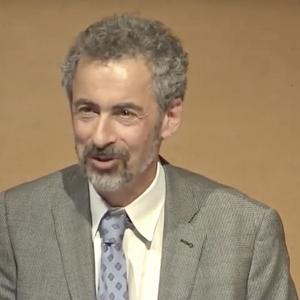
\includegraphics[width=0.68\textwidth]{images/portrait}
    	\end{center}
    	\href{}{Dr. David Kaplan} is a Professor of Physics at the University of Washington and is the Director of the National Institute for Nuclear Theory (INT). He received his BS in Physics from Stanford in 1980, and his PhD from Harvard in 1985 under the supervision of Howard Georgi. Prof. Kaplan then conducted his post-doctoral work while in the Harvard Society of Fellows, and then joined the faculty at UC San Diego in 1989. He moved to Seattle as a Senior Fellow at the INT in 1994, where he became Director in 2006. Kaplan is a Member of the National Academy of Sciences and the American Academy of Arts and Sciences, and the Washington State Academy of Sciences, and is a Fellow of the American Physical Society. He is the recipient of the Department of Energy's Outstanding Junior Investigator Award, the National Science Foundation Presidential Young Investigator Award and the Alfred P. Sloan Fellowship.
    \end{block}


%%%%%%%%%%%%%%%%%%%%%%%%%%%%%%%%%%%%%%%%%%%%%%%%%%%%%
%            BLOCK: RESEARCH INTERESTS              %
%%%%%%%%%%%%%%%%%%%%%%%%%%%%%%%%%%%%%%%%%%%%%%%%%%%%%
    \begin{block}{Research Interests}
        Kaplan has worked in various aspects of particle theory, including electroweak baryogenesis, the asymmetric dark matter paradigm, and the composite Higgs mechanism. In lattice field theory Kaplan helped solve the problem of how to simulate fermions without destroying their chiral symmetry, in effect representing the four-dimensional world as the boundary of a five-dimensional topological insulator. 
        \begin{center}
	    	
\includegraphics[width=0.65\textwidth]{images/research}    		

    	\textit{Depiction of a lattice used for calculation.} 
    	\end{center}

    \end{block}
\end{column}
\begin{column}{0.55\textwidth - 1cm}


%%%%%%%%%%%%%%%%%%%%%%%%%%%%%%%%%%%%%%%%%%%%%%%%%%%%%
%                 BLOCK: ABSTRACT                   %
%%%%%%%%%%%%%%%%%%%%%%%%%%%%%%%%%%%%%%%%%%%%%%%%%%%%%
    \begin{block}{Talk Abstract}
    	Chiral symmetries play an important role in the spectrum and phenomenology of both the standard model and various theories for physics beyond the standard model. In many cases chiral symmetry is associated with nonperturbative physics which can only be quantitatively explored in full on a lattice.
    \end{block}


%%%%%%%%%%%%%%%%%%%%%%%%%%%%%%%%%%%%%%%%%%%%%%%%%%%%%
%                BLOCK: BACKGROUND                  %
%%%%%%%%%%%%%%%%%%%%%%%%%%%%%%%%%%%%%%%%%%%%%%%%%%%%%
    \begin{block}{Brief Background}
    	Chiral symmetry is the spontaneous symmetry breaking of the chiral symmetry of the fermions in gauge theories like Quantum Chromodynamics. 
    	In quantum field theory, the left handed and the right handed fermions are decoupled and obey a global SU)3)xSU(3) symmetry. But such a symmetry prevents the quarks to have mass terms in the Lagrangian. Under spontaneous symmetry breaking the symmetry breaks down to a diagonal SU(3) flavor symmetry thereby generating eight goldstone bosons which we understand as the pseudo scalar mesons of the theory. \cite{kaplanChiralSymmetryLattice2012}
  
    	%\cite{longLocalAxonalConduction2020} 
        \begin{center}
		   	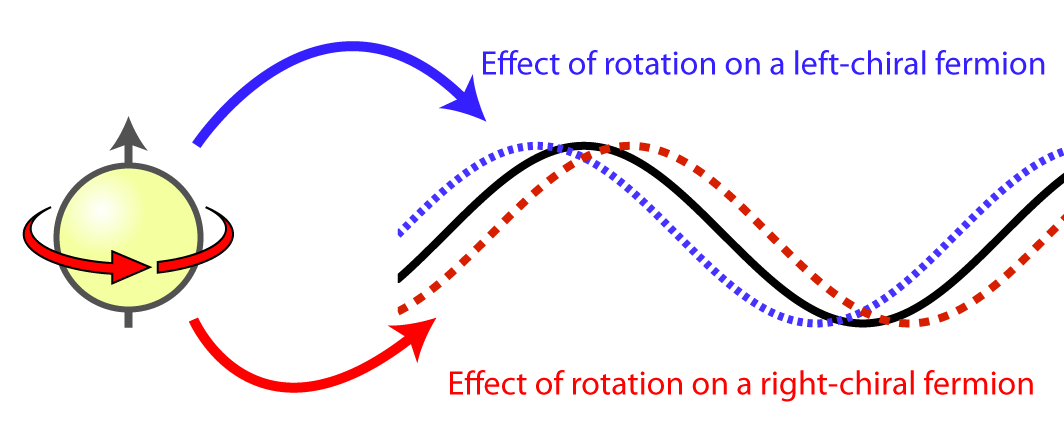
\includegraphics[width=0.95\textwidth]{images/background}    		
		
		\textit{Rotating a fermion shifts its quantum wavefunction. Left- and right-chiral fermions are shifted in opposite directions. \cite{cokerChiralsymmetry}}
    	\end{center}
    	
    	The implementation of chiral symmetry on the lattice is a nontrivial issue. In particular, local lattice fermion actions with the chiral symmetry of the continuum theory suffer from the fermion doubling problem. The Ginsparg–Wilson relation implies Lüscher’s lattice variant of chiral symmetry which agrees with the usual one in the continuum limit. Local lattice fermion actions that obey the Ginsparg–Wilson relation have an exact chiral symmetry, the correct axial anomaly, they obey a lattice version of the Atiyah–Singer index theorem, and still they do not suffer from the notorious doubling problem. \cite{chandrasekharanIntroductionChiralSymmetry2004}
    	
		%\cite{longMorphologicalCharacterizationHVC2018} 
    \end{block}


%%%%%%%%%%%%%%%%%%%%%%%%%%%%%%%%%%%%%%%%%%%%%%%%%%%%%
%                 BLOCK: REFERENCES                 %
%%%%%%%%%%%%%%%%%%%%%%%%%%%%%%%%%%%%%%%%%%%%%%%%%%%%%
    \begin{block}{References}
        \bibliographystyle{aipnum4-1}
%        \bibliographystyle{iopart-num}
		\bibliography{references}
    \end{block}

\end{column}
\end{columns}


%%%%%%%%%%%%%%%%%%%%%%%%%%%%%%%%%%%%%%%%%%%%%%%%%%%%%
%                    FOOTER TEXT                    %
%%%%%%%%%%%%%%%%%%%%%%%%%%%%%%%%%%%%%%%%%%%%%%%%%%%%%
\begin{textblock}{0.5}(0.18, 0.94)
    \color{white}
    \sffamily
    \textbf{Eberly College of Science}
    \\
    Department of Physics
\end{textblock}


%%%%%%%%%%%%%%%%%%%%%%%%%%%%%%%%%%%%%%%%%%%%%%%%%%%%%
%                   END TEMPLATE                    %
%%%%%%%%%%%%%%%%%%%%%%%%%%%%%%%%%%%%%%%%%%%%%%%%%%%%%
\end{frame}
\end{document}
